\chapter{Introduction}
\section{Overview}
This project provides a framework with which the dynamics of
an epidemic event composed of multiple, overlapping sub-epidemics may be modelled and
forecasted in real time. We aim to provide an optimised model fit to a
given set of epidemic data where all model parameters are assumed to
be unknown. The challenge of considering various candidate model
types is also considered. Unlike previous approaches, the presented framework is
implemented in object oriented style using a general purpose
programming language, allowing improved customisability and
speed. Furthermore, we attempt to implement a maximum likelihood based
fitting procedure, which has previously only been considered for
single epidemic models.

\section{Motivation}
Epidemic spreading processes can be observed in a wide range of
fields. Any type of interaction between individuals will allow the
propogation of ideas or parasites through a population, with some spreading
processes arising unexpectedly in excess of baackground levels. In the case of
infectious diseases, such outbreaks are termed epidemics. Indeed, many significant
historical events have been heavily influenced by epidemics, and the
WHO estimates that infectious diseases account for more than 13
million deaths per year.\cite{who} It is therefore no wonder that
epidemiology, the study of the mechanisms and population dynamics of
infectious diseases, has become a central field of research. With the
advancement of computing technology and methodology, new opportunities
to develop complex mathematical and computational models of real-time
epidemics have emerged.

Although the study of infectious disease spread continues to be an
area of particular research focus, globalisation and advances in
communication technologies have led to a new and rapidly developing
type of internet based epidemic. With the entire world connected
online, new ideas, trends and information can disseminate through the
world wide web almost instantaneously, and as these spreading
processes become increasingly central to modern day life, interest
from academic, commercial and social fields continues to increase. One
highly relevant theory is that of `memes' as proposed by Richard
Dawkins, who suggests that ideas, behaviours and styles spread like
"mind viruses" between individuals within a culture.\cite{dawkins} The
adaptation of this term to describe the spread of fads on the internet
demonstrates the relevance of studying the dynamics of epidemic
processes over the internet. \cite{meme}

Research into the dynamics of internet-based phenomena are largely at
an early stage, and have mostly focused on Online Social Networks
(OSNs) such as Facebook and Twitter, and content sharing websites such
as YouTube.\cite{hartmann, bieber} The analogy between infectious
diseases and the spread of content online is easy to consider: the
social networks formed on OSNs simulate physical interactions in real
life as users interact and share content on their profiles, whilst
viewing and subsequently sharing a YouTube video may be compared to
contracting and spreading an infectious disease. There is a growing
body of research that aims to use ideas from epidemiology to better
understand the spread of internet-based phenomena. \cite{marily2013,
  meme, wang} Taking inspiration from epidemiology, the study of
internet-based epidemic phenomena has investigated the applicability
of both locally and globally driven models. For example, some studies
have investigated the use of diffusion models to describe the
disemmination of influence, whilst others have investigated the use of
global mathematical models.\cite{marily2013, meme, wang, hu}

Whilst these studies have shown generally promising results, a recent
study highlighted the limitations of the single epidemic based
approach.\cite{marily2013} The co-occurence and interaction between
diseases and with environmental factors is increasingly realised as
important, and the authors suggest that the corresponding field of
\emph{synepidemiology} can be applied to internet-based
epidemics.\cite{singer, bastos} The authors go on to coin the term
\emph{synthedemics} to describe the co-occurence of a set of
infections that may or may not be dependent on each
other.\cite{marily2014} Taking inspiration from Fourier analysis, the
study goes on to investigate how an incoming epidemic signal can be
broken down and described in terms of multiple epidemic components
(Figure 1). Furthermore, the authors build on a previous study to
allow models to be fit in real time without making assumptions
regarding the initial model parameters.




 \begin{figure}[ht!]
\centering
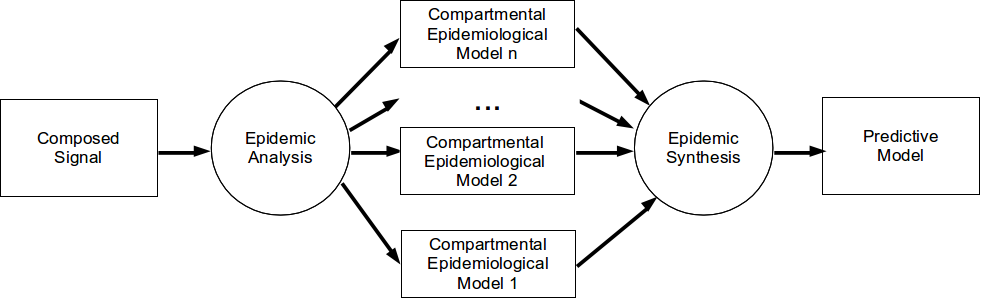
\includegraphics[width=140mm]{marily2014.png}
\caption{Model construction framework as proposed by Nika et al. 2014.\cite{marily2014}}
\label{sir}
\end{figure}

\section{Objectives}
The aim of this project is to implement a real time model fitting
framework with which epidemic phenomena might be characterised and
forecasted. When provided with epidemic data up to an arbritary time point,
we attempt to fit an appropriate number of sub-epidemics of various
types to best describe the current data, and to allow future time
points to be predicted. The course of the project can be split up into
the following sub goals:

\subsection{Single Epidemics}
The first objective of this project is to implement a single epidemic
fitting framework, treating the growth and recovery rates of the
epidemic as unknown parameters. This framework is then extended to
additionally consider the initial number of susceptible individuals
and the actual epidemic start time as unknown parameters. The model
fitting procedure is undertaken using optimisation with both least
squares and maximum likelihood estimations. The framework allows for
`on the fly' fitting, such that a model may be fit to the data as the
epidemic unfolds and more data points are obtained.

The initial implementation of this framework is initially undetaken using the R
statistics programming environment due to the availability of useful
packages and functions. For example, the \emph{deSolve} for solving
first-order ordinary differential equations (ODEs), the \emph{optim}
function for optimising a set of model parameters, and the
\emph{bbmle} package for maximum likeliihood based fitting.

An extension of this objective that arose during the course of the
project is the implementation of the fitting framework in C++ `from
scratch'.

\subsection{Multiple Epidemics}
Not all epidemic phenomena are constrained to a single population, and
the single epidemic fitting methodology is therefore inadequate in
characterising all epidemics. For example, the measure of
\emph{YouTube} video views over time might be composed of multiple
spikes of interest as the video is shared in new online social
groups. This limitation also affects to infectious disease dynamics,
wherein the total number of infected individuals in a country might be
affected by the penetration of the disease into different cities. The
second objective of this project is therefore to implement a model
fitting framework that can simultaneously fit and combine multiple
sub epidemics into a single model. 

As in the single epidemic fitting framework, the multiple epidemic
fitting framework makes no assumptions regarding model parameters such
as growth rate, recovery rate, start time and number of
susceptibles. As above, an initial implementation will be attempted
using R. However, as the computational difficulty of fitting
multiple sets of parameters simultaneously increases as the number of
sub epidemics increases. We therefore provide a final `from scratch' implementation in C++.

A significant extension of this fitting methodology is to allow
different epidemic models to be considered. That is, which one of a
number of model equations can be used to best describe the data? An
object-oriented C++ implementation is therefore provided to consider
the addition and removal of various candidate models to describe a set
of data.

\subsection{Maximum Likelihood Estimation}
A novel objective of this project is to use maximum likelihood rather
than least squares to find an optimised model fit. A significant
challenge of this is to implement an efficient likelihood function in
C++ with which a set of parameters might be optimised in reasonable
time. An advanced extension of this objective is to generate confidence
intervals characterise uncertainty in the optimised parameters. 

\subsection{Evaluation}
All of the above objectives must be validated, and we use a
number of data sources to assess the model fitting
framework. Synthetic data provides the core of the evaluation, as it
allows for the retrieval of known parameters from artificially
generated data. Finally, we consider the framework's ability to
provide model fits to historic infectious disease data and online
epidemic phenomena.

\section{Contributions}

Contributions here.


\section{Report Structure}

Statement here.
